%Sample Headers:
%Introduction and objectives
%Background information and previous work in the subject area (referenced)
%Theoretical aspects/modelling/simulation/strategies
%Experimental techniques/methods/apparatus/rationale
%Results
%Discussion of results/critical analysis/comparison with other work
%Suggestions for future work
%Conclusions
%References
%Appendices (equations/program code/equipment specifications)
%Logbook (for Teaching Periods 1 and 2 – ensure there is an entry for every week)

\chapter{Summary of achievements to date}

\begin{itemize}
\itemsep1pt\parskip0pt\parsep0pt
\item
  The author has familiarised himself with relevant communications
  theory, including modulation schemes, probability theory and optimum
  detector design.
\item
  The author has become acquainted with the Mathematica programming
  environment and used it to program a number of mathematical
  simulations describing communications problems.
\item
  The author has examined the effects of receiver timing error on BPSK
  and 4-PAM signalling schemes using root raised cosine filters, and
  demonstrated sub-optimal detection performance with 4-PAM using
  standard detector designs and assuming a memoryless communications
  channel with additive white Gaussian noise.
\item
  The author has characterised the change of optimum decision region
  boundaries in the presence of non-deterministic timing errors
  following a known probabilistic model.
\item
  A clear plan of work for the first half of Teaching Period 2 has been laid out,
  and is expected to centre around the effects of timing error offset in the
  presence of Rayleigh fading.
\end{itemize}

\ctparttext{A description of the project, including an explanation of the underlying theory, followed by a summary of the work undertaken to date.} 

\part{Project Description}

\chapter{Introduction and background to the project}

This project seeks to examine the effects of receiver timing error in
radio communications systems. Understanding how radio system performance
decreases in sub-optimal conditions is key to assessing a system's
performance and designing more robust and better performing radio systems. The
principle goal is to be able to characterise the effects of timing error such
that a receiver may be optimised to account for it.

A typical radio communications system consists of a transmitter, a
receiver and a communications channel, that may contain any number of
non-idealities. For this reason, if a transmitter sends a particular
symbol down a real communications channel, the received symbol may be
substantially different to the sent symbol. Therefore, careful attention
is required to the design of the receiver symbol detector.

One could imagine a binary transmission system that sends one of two
possible signals: a 1V$_{RMS}$ wave if a `0' is to be sent, and a
3V$_{RMS}$ if a `1' is to be sent. After being distorted by the
communications channel, the receiver could in theory see a signal of any
amplitude, and must make a decision as to which amplitude was originally
sent. It would be helpful to know the probability density function (PDF)
of the received signal, ie. the probability of receiving a signal
amplitude if a known amplitude was sent. If one assumes the communications
channel is memoryless and distorts the signal by adding zero-mean white Gaussian noise,
the received signal PDF will be a Gaussian distribution centred on the
sent signal amplitude, as shown below. If both symbols are equiprobable, their PDF's will be of equal height, and therefore shifted copies of each other.

\begin{figure}[htbp]
\centering
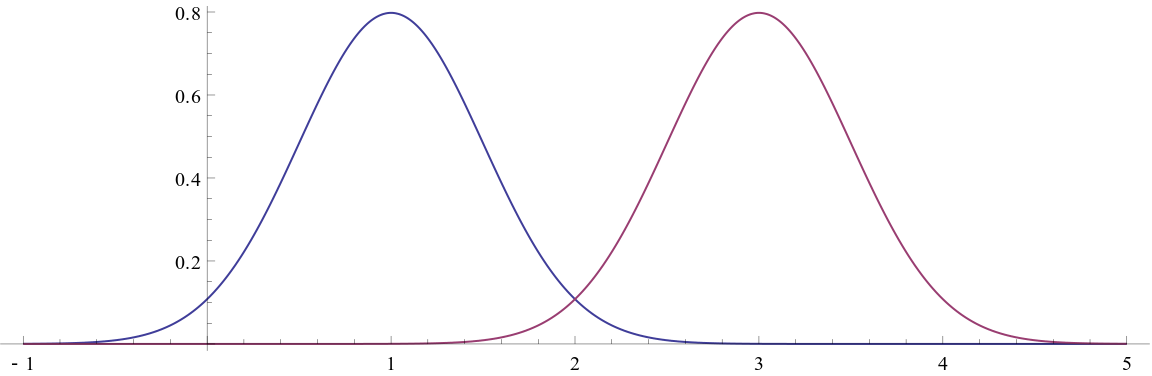
\includegraphics[width=\linewidth]{4-PAM_PDF.png}
\caption{Gaussian noise corrupts a sent signal, resulting in a
probability density function for each possible sent symbol}
\end{figure}

\begin{figure}[htbp]
\centering
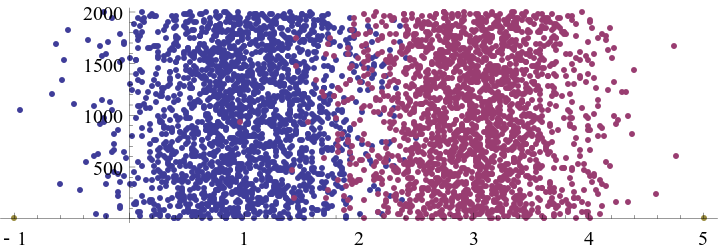
\includegraphics[width=\linewidth]{4-PAM_samples.png}
\caption{As an example, 2000 of each symbol has been send down the
communications channel. The received values distorted by noise are
plotted above. Note the overlap in received values corresponding to both
symbols: it is impossible to detect the signal with 100\% accuracy.}
\end{figure}

A \emph{maximum-likelihood (ML) detector} seeks to minimise the probability of
error by always picking whichever signal was most likely to be sent, given
the received signal. Therefore, the threshold between picking one value or the other
will be where both symbols are equally likely to be sent, the point of
intersection of both PDF's. Since the Gaussian distribution is symmetric
about its mean, in this case the threshold (or \emph{Decision Region
Boundary}) is exactly midway between both sent amplitudes. Intuitively
this makes sense: it says that in the simplest case if one receives a particular
signal, one should assume whichever possible sent signal is nearest. However in more complicated cases picking the point of intersection of both PDF's
is a more general solution. 

One issue that complicates detection is \emph{inter-symbol
interference} (ISI). It is possible for signals representing symbols in
the future or past to bleed into the current symbol clock period,
distorting the signal further. For this reason transmitters and receivers
are designed such that they apply a \emph{raised cosine function} that
is fully transparent at exactly the symbol's sample time, and blocks
completely at every other symbol's sample time, ie at every interval of
$T_{clk}$ for $T \neq 0$. If both receiver and transmitter are perfectly
synchronised, this ensures that the receiver will only see signals
corresponding to the current transmitted symbol, after distortion via
the communications channel.

\begin{figure}[htbp]
\centering
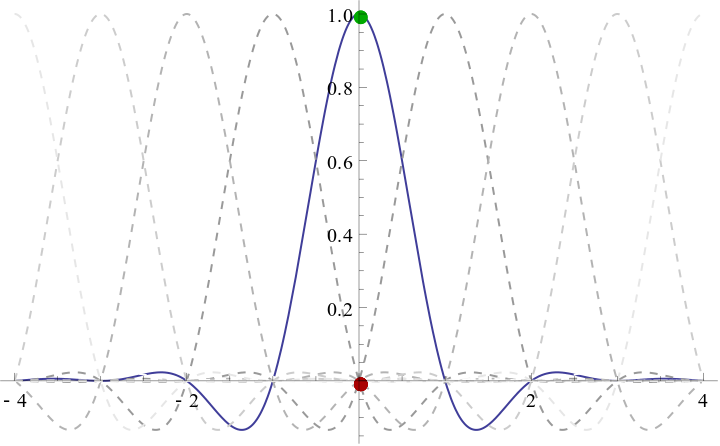
\includegraphics[width=\linewidth]{rrc_sync.png}
\caption{A filter with a root raised cosine function is often used, as
it evaluates to 1 at the current sample time and 0 at all other sample
times}
\end{figure}

\begin{figure}[htbp]
\centering
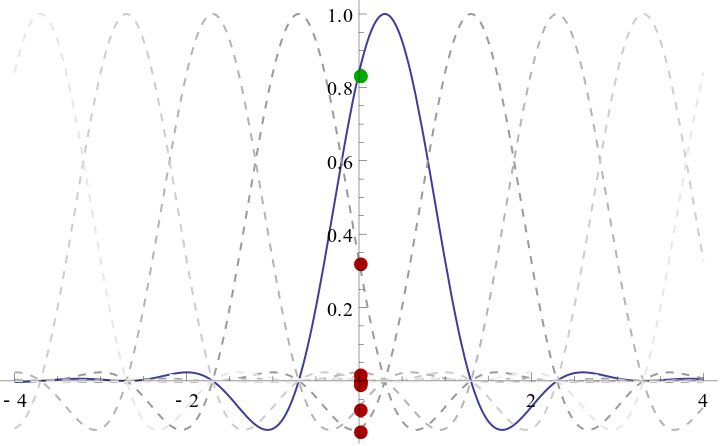
\includegraphics[width=\linewidth]{rrc_err.png}
\caption{If a timing offset is added to the root raised cosine it no
longer evaluates to 0 or 1 at the sampling time. This results in
reduced receiver performance when the receiver and transmitter are not
properly synchronised.}
\end{figure}

If the receiver and the transmitter are poorly synchronised, however,
the root cosine filter response is shifted in time with respect to the
receiver and looses some of its essential property. Current literature
has considered the effects of a Tikhonov-distributed timing offset in a Nagakami-\emph{m} channel with rectangular signalling and diversity combining \cite{[2]}, and a uniformly distributed timing offset in a Rayleigh fading channel \cite{[6]}. The effects of timing offset in the BPSK and QAM cases have been studied in \cite{[3]} \& \cite{[4]}, and \cite{[5]}, respectively However, the effects of a poorly synchronised receiver on detection performance in the root-cosine filter case has not to date been published. This project seeks to examine this matter further, and ascertain whether design decisions can be made to mitigate its effects.

\chapter{Description of the project}

The author started by researching the underlying theory. \cite{[8]} was used as a reference textbook, and explains probability theory and optimum receiver design. The concepts of representing non-deterministic signals using probabilistic models,  maximum-likelihood (ML) and maximum a posteriori (MAP) receivers and designing optimum receivers given a known probabilistic model for the receiver, were studied in depth. In addition, a method for estimating received signal PDF's with a Gram-Charlier PDF developed by UCC graduate David McCarthy in \cite{[1]} was studied. Finally, the Mathematica language had to be learnt from scratch, with emphasis on statistics and plot generation.

In order to familiarise myself further with these concepts, I built a
simple model for a two-symbol BPSK communications system in Mathematica.
I extended this to the 4-symbol 4-PAM system. With some help from David I also
implemented the Gram-Charlier distribution. Using these programs as a
base I then wrote a simulation that can produce a PDF of the receiver input
with a known timing offset. Using this, I was able to examine how the
sent symbol is distorted by the channel and timing error, and found that
increasing amounts of offset reduced the effective amplitude of the
signal while increasing noise due to ISI. Additionally, it was found
that the optimum decision region boundary was decreased by a factor
equal to the value of the root raised cosine function at the timing
offset.

My attention at this stage turned to increasing the speed of the
simulations, and much work was done studying Mathematica's potential for
parallelisation. I was able to acquire remote access to a number of Unix
machines, and ported the simulations to run across multiple machines,
paying attention to taking advantage of the dual-core processors and
making the code resilient to premature termination (due to power outages,
illiterate students etc.).

A more realistic model was created by assuming that the timing error is
not a fixed value, but could be described by a Tikhonov distribution.
Two approaches were taken: an initial, quick approach was to calculated
the optimum decision region boundary of each timing error, and average
this over the probability of each timing error occurring. This assumes
that multiple possible optimum decision region boundary locations could
be averaged to give the overall optimum decision region boundary
location, which I learnt was not generally the case, and this was later
proven analytically by David. I therefore tried a second, more realistic
approach, where for each simulated transmission a new timing offset was
chosen from the Tikhonov distribution. An optimum decision region
boundary was then determined for multiple Tikhonov distribution widths
(or variances). It was found that the optimum decision region boundary
decreased as the variance of the Tikhonov distribution increased.

\begin{figure}[htbp]
\centering
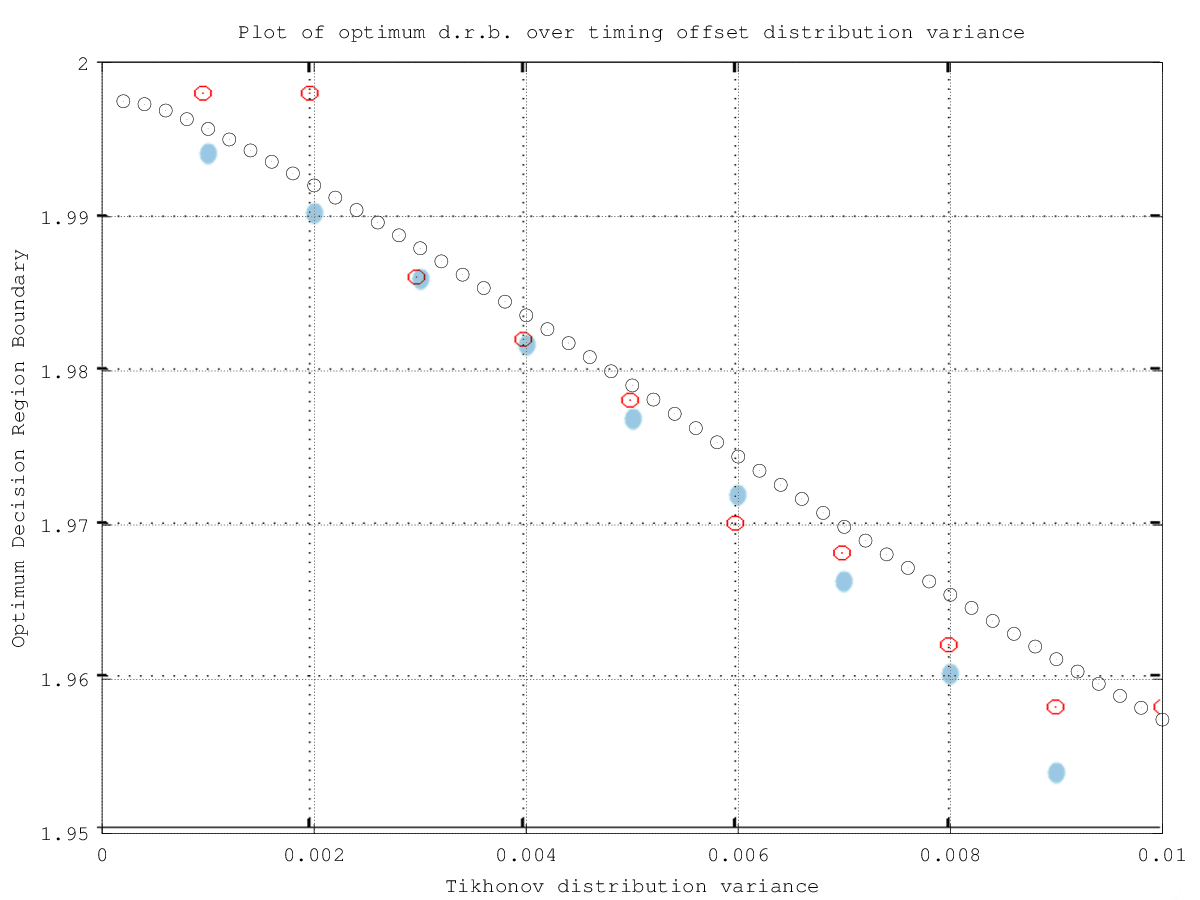
\includegraphics[width=\linewidth]{../../../plots/opt_dec_reg.png}
\caption{Optimum Decision Region Boundary for various timing error
probability distributions. Black: estimate found by averaging fixed timing errors over Tikhonov distribution; Blue: analytical result determined by Dave; Red: simulation results.}
\end{figure}

To summarise, my work in TP1 helped introduce me to radio communications
systems, and concepts of signal corruption and optimum detectors. I
learnt how to translate signal transmission into mathematical
simulations, and how to extract meaningful conclusions from the output.
Using the theory and simulations developed during this time I was able
to demonstrate a changing optimum decision region boundary in the
presence of a non-deterministic timing offset using 4-PAM signalling. It
is believed this behaviour can be generalised to L-PAM signalling. \marginpar{By \emph{L-PAM} I mean PAM signalling with an arbitrary number L of possible symbols. L=4 reduces to 4-PAM.} This will serve as a foundation from which to explore the effects of a
non-deterministic timing offset in more general cases.

\ctparttext{A plan of work for Teaching Period 2, and a brief discussion of ethical issues pertaining to the project.} 

\part{Going Forward}

\chapter{Plan for Teaching Period 2}

In TP2, the author aims to extend the scope of the project to address the issue of
timing error offset in communications channels subject to fading effects
such as in urban areas or for very long-range communications. In either
case, line-of-sight communication is very weak or non-existent, and the
signal is scattered and received as a combination of multiple
"bounced" signals with different propagation delays and amplitudes. In order to improve reception in this case, the signals from multiple antennas are combined before being presented to the symbol detector. I will model these using a Rayleigh distribution, and assuming an Equal Gain Combining (EGC or additive) receiver, determine the effects of
timing error described above on this type of model. the decision has been made to stick to
L-PAM signalling, as PSK signalling formats rely solely on phase
detection and therefore the optimum decision region boundaries are
unaffected by amplitude changes.

Once a description of the optimum detector in the presence of
Rayleigh fading has been formulated, the next goal will be to compare it to the optimum
detector described in \cite{[2]}, which assumes perfect
synchronisation (ie. no timing offset).

A project plan is presented here as a guide to how work is expected to
proceed in TP2. This plan is to be considered a mere guide, as no project plan can be accepted as gospel truth (Hopfstadter's Law \cite{[11]}, among others). In order to account for this timescales have been made purposefully conservative. This plan purposely only covers up to mid-February, as the results of the work below will dictate the direction to take the project in during the second half of TP2, therefore the author is unable to predict with reasonable certainty what work will be carried out.

\begin{landscape}
\begin{longtable}[c]{@{}llll@{}}
\hline\noalign{\medskip}
\begin{minipage}[b]{0.2\columnwidth}\raggedright
Description
\end{minipage} & \begin{minipage}[b]{0.1\columnwidth}\raggedright
Time Allowed
\end{minipage} & \begin{minipage}[b]{0.1\columnwidth}\raggedright
Start Date
\end{minipage} & \begin{minipage}[b]{0.46\columnwidth}\raggedright
Goals
\end{minipage}
\\\noalign{\medskip}
\hline\noalign{\medskip}
\begin{minipage}[t]{0.2\columnwidth}\raggedright
Review of Rayleigh fading
\end{minipage} & \begin{minipage}[t]{0.1\columnwidth}\raggedright
1 week
\end{minipage} & \begin{minipage}[t]{0.1\columnwidth}\raggedright
6 Jan
\end{minipage} & \begin{minipage}[t]{0.46\columnwidth}\raggedright
\begin{itemize}
\itemsep1pt\parskip0pt\parsep0pt
\item
  Develop an understanding of Rayleigh fading.
\item
  Have built a basic Mathematica model of Rayleigh fading assuming
  perfect synchronisation.
\end{itemize}
\end{minipage}
\\\noalign{\medskip}
\begin{minipage}[t]{0.2\columnwidth}\raggedright
Implement Rayleigh fading model with timing error
\end{minipage} & \begin{minipage}[t]{0.1\columnwidth}\raggedright
1 week
\end{minipage} & \begin{minipage}[t]{0.1\columnwidth}\raggedright
13 Jan
\end{minipage} & \begin{minipage}[t]{0.46\columnwidth}\raggedright
\begin{itemize}
\itemsep1pt\parskip0pt\parsep0pt
\item
  Extend previous model to account for timing errors following a
  Tikhonov distribution model.
\item
  Evaluate optimum decision region boundary in the presence of timing
  error offsets and Rayleigh fading.
\end{itemize}
\end{minipage}
\\\noalign{\medskip}
\begin{minipage}[t]{0.2\columnwidth}\raggedright
Additional simulation time
\end{minipage} & \begin{minipage}[t]{0.1\columnwidth}\raggedright
1 week
\end{minipage} & \begin{minipage}[t]{0.1\columnwidth}\raggedright
20 Jan
\end{minipage} & \begin{minipage}[t]{0.46\columnwidth}\raggedright
\begin{itemize}
\itemsep1pt\parskip0pt\parsep0pt
\item
  Characterise the effect of non-deterministic timing error on the
  optimum decision region boundary for L-PAM signalling in the presence
  of Rayleigh fading.
\end{itemize}
\end{minipage}
\\\noalign{\medskip}
\begin{minipage}[t]{0.2\columnwidth}\raggedright
Compare described receiver to optimum receiver described in literature
\end{minipage} & \begin{minipage}[t]{0.1\columnwidth}\raggedright
2 weeks
\end{minipage} & \begin{minipage}[t]{0.1\columnwidth}\raggedright
27 Jan
\end{minipage} & \begin{minipage}[t]{0.46\columnwidth}\raggedright
\begin{itemize}
\itemsep1pt\parskip0pt\parsep0pt
\item
  Provide a detailed comparison of the optimum described above, to the
  optimum receiver described in \cite{[2]}, paying particular
  attention to performance in the presence of non-deterministic timing
  error.
\end{itemize}
\end{minipage}
\\\noalign{\medskip}
\hline
\end{longtable}
\end{landscape}

\begin{landscape}
\begin{figure}[ftbp]
\begin{center}

\begin{ganttchart}[y unit title=0.5cm,
y unit chart=0.5cm,
vgrid,hgrid, 
title label anchor/.style={below=-1.6ex},
title left shift=.05,
title right shift=-.05,
title height=1,
bar/.style={fill=gray!50},
incomplete/.style={fill=white},
progress label text={},
bar height=0.7,
group right shift=0,
group top shift=.6,
group height=.3,
group peaks={}{}{.2}]{35}
%labels
\gantttitle{Jan}{26} 
\gantttitle{Feb}{9} \\
\gantttitlelist{6,...,31}{1} 
\gantttitlelist{1,...,9}{1}\\
%tasks
\ganttbar{Review}{1}{7} \\
\ganttbar{Implement}{8}{14} \\
\ganttbar{Simulations}{15}{21} \\
\ganttbar{Comparison}{22}{35}
%relations 
\ganttlink{elem0}{elem1} 
\ganttlink{elem1}{elem2} 
\ganttlink{elem2}{elem3} 
\end{ganttchart}
\end{center}
\caption{Gantt Chart}
\end{figure}
\end{landscape}

\chapter{Discussion of ethical issues}

In communications systems, as in any area seeing considerable
technological developments, the question of whether these developments
are ethically sound naturally arises. The advent and spread of radio
throughout the 20th century brought about an era of increased
connectedness and information transfer, as information could be rapidly
spread across large distances with little effort. The advent of the
internet in 1969 and the mobile phone
boom of the 90s accelerated these changes as almost-instant,
asynchronous and on-demand information transfer became available to the
general public, and current Web 2.0 developments such as social
networking are but continuations of this trend. With the smart-phone
industry putting internet access into the pockets of consumers, many
believe that these changes, driven by advances in communications
technology, have had a considerable impact on our societies. While the
positives are too numerous to note, the skeptic would also readily see
the disadvantages.

Engineering developments can lend themselves to applications with both
positive and negative intentions, as with any scientific advancement.
Radio technology developments in particular has throughout history been
closely linked to the military.
Improving wireless communications can play into the hands of military
and terrorist leaders, as cheap and reliable wireless communications can
aid the organisation and execution of manoeuvres. In addition the remote
detonation of explosives using mobile phones is considered a real threat
to many cities \cite{[10]}. Therefore, communications research enters the same ethics discussion as other defence research.

These same developments have created privacy concerns as most citizens find themselves communicating daily through the internet and the cell phone network. At the bottom of the internet hierarchy, endpoint routers are naturally trusting, and prone to exploitation; in addition, they are generally visible to all other internet users. At the top, most communications are routed through a small number of Tier 1 networks, which have proven themselves prone to eavesdropping. As the distance over which an individual can send a piece of information to its intended recipient has increased, so has the number of individuals capable of intercepting this information. Thus as users embrace the internet and smart phones, they also find themselves increasingly exposed to spying from a number of groups with varying intentions. Even outside of the "online" world, increasing the efficiency of radio receivers can lead to the exploitation of security-sensitive short-range communications. For example, contactless payment devices rely on short range communications to transfer identification information for payment purposes. Equipped with a suitable exploit, such as described in \cite{[9]}, a high-accuracy receiver would increase the number of these devices in range of an attacker.

The author notes that these issues relate to the broad area of communications within which this project falls. However he does not feel there is a direct ethical concern with any of the work described within here.
